\section{Background}


\subsection{Basic Failure Model in Reliability Study}

In reliability study, the time when the first failure occurs in often assumed 
to follow a probability density function (pdf) if time is a continuous value, or 
a probability mass function (pmf) if time is a discrete value. \citep{MusaBook} 
 
The value of time is a continuous value if its unit is a {\it time unit} (e.g. 
second) and the value could be any real number.  The value of time is 
a discrete value if its unit is a {\it natural unit} (e.g. number of 
operations) or its unit is a {\it time unit} but the user only cares the 
status of a system at discrete time (e.g. every second).

Although the precise definition of failure varies in different systems, 
measures of failures can be consistently defined in terms of a pdf or a
pmf.  Assuming that the pdf of a system is $f(t)$, measures of failures can be 
defined as in Figure \ref{eq:measure_of_failures} 
\citep{MusaBook}.  Measures of failures can be defined in terms of pmf 
similarly.

\begin{figure}
\begin{subequations} 
\begin{align}
    R(t) & = \int_{t}^{\infty} f(x) dx = 1- \int_{0}^{t} f(x) dx  \label{subeq1}\\
   MTTF & = \int_{0}^{\infty} tf(t)dt  = \int_{0}^{\infty} R(t)dt 
\label{mttf}\\
   h(t) & = \lim_{\Delta t\rightarrow 0} \frac{R(t)-R(t+\Delta t)}{\Delta t 
R(t)}  = \frac{f(t)}{R(t)}
\end{align}
\end{subequations}
\caption{Measures of Failures}
\label{eq:measure_of_failures}
\end{figure}

In the above, the reliability during a specific time, $R(t)$, is the 
probability that a system can survive without failure throughout that time.  
The Mean Time to Failure (MTTF) is the average time when the first failure 
occurs.  The hazard rate at time $t$ is the failure rate at that time given 
the condition that the system has survived for $t$ time.  Equation 
\ref{failure_check} checks that the average failure rate ($\lambda$) is the 
reciprocal of MTTF.

\begin{equation}
 \lambda = \int_{0}^{\infty} h(t) dt = \int_{0}^{\infty} \frac{f(t)}{R(t)}  dt 
=  \frac{\int_{0}^{\infty} f(t) dt}{\int_{0}^{\infty} R(t) dt} = \frac{1}{MTTF}
\label{failure_check}
\end{equation}




\subsection{Traditional Software Rejuvenation Models}

\subsubsection{The Basic Model}


The basic software rejuvenation model proposed by
\citep{huang1995software} is modelled by the state transition diagram in 
Figure \ref{fig:model_classic_1}.  Huang et. al defines the following 4 states:

\begin{description}
  \item[S] The robust {\tt start} state in which the system will not fail.
  \item[W] The failure probable {\tt working} state in which the system may 
fail at a certain probability.
  \item[F] The {\tt failure} state when the system reaches its boundary condition.
  \item[R] The {\tt rejuvenation} state when the system is plan to 
restart to a clean state.
\end{description}

\citep{huang1995software} decides the rejuvenation thresholds using the 
following process.  

\begin{enumerate}
  \item compute the probabilistic {\it mean} rates of every state transitions 
somehow.
  \item calculate the probability of the system being in each state, based on 
the state transition rates computed above.
  \item calculate the {\it expected} total time of the system in state $s$ 
during an interval of $L$ time units as $T_s(L) = p_s \times L$, where $p_s$ is 
the probability the system being in state $s$ calculated in the second step.
  \item calculate the cost of downtime during interval $L$ as $Cost(L) = (p_f 
\times c_f + p_r \times c_r) \times L$, where $p_f$ and $p_r$ are probabilities 
the system in state $F$ and $R$ respectively, and $c_f$ and $c_r$ are unit cost 
of the system in state $F$ and $R$ respectively.
  \item determine the optimal rejuvenation thresholds by finding the optimal 
transition rate between state $W$ to state $F$ so that the cost of downtime is 
minimum.
\end{enumerate} 

The original software rejuvenation model, proposed by 
\citet{huang1995software}, has shown its significance in long running billing 
systems, scientific applications, and telecommunication systems 
\citep{huang1995software}. Readers may have noticed that the above estimation 
methodology gives an approximate statistical estimation for a long running 
system because the usage of {\it mean} state transition rates and the {\it 
expected} time of being in each state.  By {\it long running system}, we refer 
to a system whose expected in-service time is a statistically long time regards 
to its MTTF, repair time, and rejuvenation time.


\begin{figure}
  \centering         
        \subfigure[Traditional Model 1]{
            \label{fig:model_classic_1}
            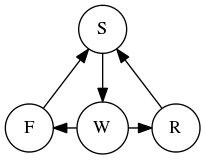
\includegraphics[scale=0.5]{model_1.png}
        }\\
        \subfigure[Traditional Model 2]{
            \label{fig:model_classic_2}
            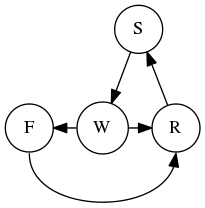
\includegraphics[scale=0.5]{model_2.png}
        }\\
    \caption{Traditional Software Rejuvenation Models}
   \label{fig:model_traditional}
\end{figure}

\subsubsection{A Modified Model}

\citet{dohi2000statistical} modifies the original model given 
by \citet{huang1995software} with the following modifications:

\begin{enumerate}
  \item As shown in Figure \ref{fig:model_classic_2}, the completion of repair process
  is immediately followed by the software rejuvenation process.
  \item Assuming that every state transition is a stochastic processes.  For each state $S$, define a 
  probability density function $F_s(t)$, which represents the probability that the system will stay in that
  state for time $t$. 
\end{enumerate} 

The first modification is made to distinguish the process of system cleanup and process resuming
from other repair tasks, the former of which is required in both the repair process and the rejuvenation
process in practice.  The second assumption is made so that the model is a Semi-Markov process,
a well studied stochastic process with off-the-shelf analysis techniques.  Although \citet{huang1995software}
do not mention the relationship between their model and Markov process, \citet{dohi2000statistical}
show that if the modified model gives the same analysis result as the one
given in \citet{huang1995software} if (i) remove assumption 1; and (ii) assume 
that the sojourn times in all states are exponentially distributed.

\citet{dohi2000statistical} decides the optimal software rejuvenation thresholds by looking for
the one that maximise the system availability, the ratio of uptime and total time.  Same as the
methodology in \citet{huang1995software}, instead of precisely describe state transition 
probabilities, $mean$ time of staying in the {\tt start} state, the {\tt failure} state, and the
{\tt rejuvenation} state is used.  The expected time of staying the failure probable {\tt working} state
is calculated by equation \ref{mttf}.

The methodology given in \citet{dohi2000statistical}  does not give a general cost
analysis as the one in \citet{huang1995software}.  It also suffers the problem of using
$mean$ times.  Despite those two limitations, \citet{dohi2000statistical} 
derived a non-parametric statistical algorithms to estimate the optimal 
software rejuvenation thresholds that maximise the system availability, based 
on statistical complete sample data of failure times.



\begin{comment}
The basic assumption of software rejuvenation is that software systems will 
become failure-probable after a period of execution.  In other words, failure 
rate is a function about the execution time t.  In contrast, the probabilistic 
state transition model 
\url{
http://citeseerx.ist.psu.edu/viewdoc/download?doi=10.1.1.176.2557&rep=rep1&type=
pdf} (FTCS 1995, citation: 711) employs the statistical mean rate of the 
transition rate between states.  

   The same model is used in the book 
\url{http://onlinelibrary.wiley.com/doi/10.1002/9780470050118.ecse394/full} 
(published in 2007)

   The same problem appears in the model used in 
\url{http://ieeexplore.ieee.org/xpls/abs_all.jsp?arnumber=897287} (HASE 2000, 
citation: 60) and 
\url{http://ieeexplore.ieee.org/stamp/stamp.jsp?tp=&arnumber=895436} (PRDC 2000, 
citation: 90), which extends the original model to be a semi-Markov process, 
where time is a continuous value.
      

Models that use the statistical mean rate can only be used to estimate the 
expected average behaviors (e.g. downtime) over a statistically long time.  A 
more serious problem is that, treating failure rate as a constant in model 
analysis violates the basic assumption of software rejuvenation.  After all, if 
the failure rate is independent of the execution time, restarting the system 
will not help at all but increase the downtime.

The link ( http://srejuv.ee.duke.edu/papers.htm ) gives a list of papers (until 
2010) on software rejuvenation.  I am surprised that the classic general failure 
model used in reliability analysis has not been applied to the model analysis of 
software rejuvenation.
\end{comment}
